\chapter{Discussion}
\label{chap:monocentric_discussion}

\begin{flushright}{\slshape    
Our progress is narrow;\\
it takes a vast world unchallenged and for granted.}  \\ \medskip
--- J. Robert Oppenheimer~\cite{Oppenheimer:1954}
\end{flushright}


\bigskip

As we stated in the introduction, all models are fundamentally wrong -- at least
incomplete. Although is it able to reproduce key empirical regularities, the
model presented in Chapter~\ref{chap:monocentric_model} is no exception to this
rule. In the following chapter, we will enumerate some of its weaknesses, and
propose possible ways in which it could be extended.\\

Because they are trying to make sense of a complex reality with a limited number
of tools, empirical analyses are not exempt of limitations either. Before
closing this chapter, we question the validity of the current methods used to
delineate subcenters, and challenge the notion of polycentricity itself.

\section{Questioning and extending the model}
\label{sec:model}

\subsection{What the model does not say}
\label{sec:what_the_model_does_not_say}

The model makes many simplifying assumptions which allow for a better
analaytical tractability, but hide some interesting aspects of intra-urban
dynamics. Thereby, we do not pretend to explain the complexity of
urban dynamics in its entirety, but rather some aspects of it.\\ 

A first feature, hidden in the assumptions of the model, is that we do not
explain the concentration of activities in localised areas in the cities.
Rather, we take the existence of centers as granted, and do not bother with the
behaviour of firms. Of course, this is a topic worthy of investigation, and
should be studied in more depth in order to have a comprehensive understanding
of the mechanisms that shape cities.

A second limitation lies in the fact that we ignore the process of residence of
residence, and attribute households' location at random in the city instead. We
therefore set aside the problem of competition for space between households, and
a theoretical description of the spatial distribution of housing prices
(see~\cite{Gauvin:2013} for a model that explores this aspect).

Another limitation lies in the description of congestion. In a worry to
simplify the problem, we chose to adopt a macro-scale description of
traffic congestion, given by Eq.~\ref{eq:commuting_cost}. The sensitivity of the
road network to congestion is taken into account through the exponent $\mu$ and
the capacity $C$, which are assumed to be the same across the entire city. In
order to derive and compute these parameters, one would need to understand how local
patterns of congestion lead to macroscropic behaviours at the city scale. This
is, of course, a difficult entreprise:  local particularities of the layout may
have dramatic consequences on the fluidity of traffic, and congestions do
propagate through the network so that access to a given center can have an
effect on the travel to another center~\cite{Li:2015}. 

\subsection{Possible avenues}
\label{sub:possible_avenues}

Even without considering the difficult problem of modeling the behaviour of the
firms, and the way it is coupled to that of individuals, the model could be
improved in several ways. 

One first possible extension is to take the presence of public transportation
into account. Indeed, the model only considers individual vehicles, prone to
congestion, as a transportation mean.  However, the largest cities in the world
are all served by metro systems~\cite{Roth:2012}, and the share of transports
other than personal vehicles can attain $42\%$\graffito{Number from the 2013
American Community Survey} in cities like New-York. It is therefore far from
being negligible, and should be taken into account in the model. 

However, in the defense of the model as it stands, cars remain the dominant mode
of transportation in the US, as shown of Fig.~\ref{fig:transportation_mode}. The
use of alternative modes of transportation is only notable in New-York, which is
already a polycentric city.\\

\begin{figure}[!h]
    \centering
    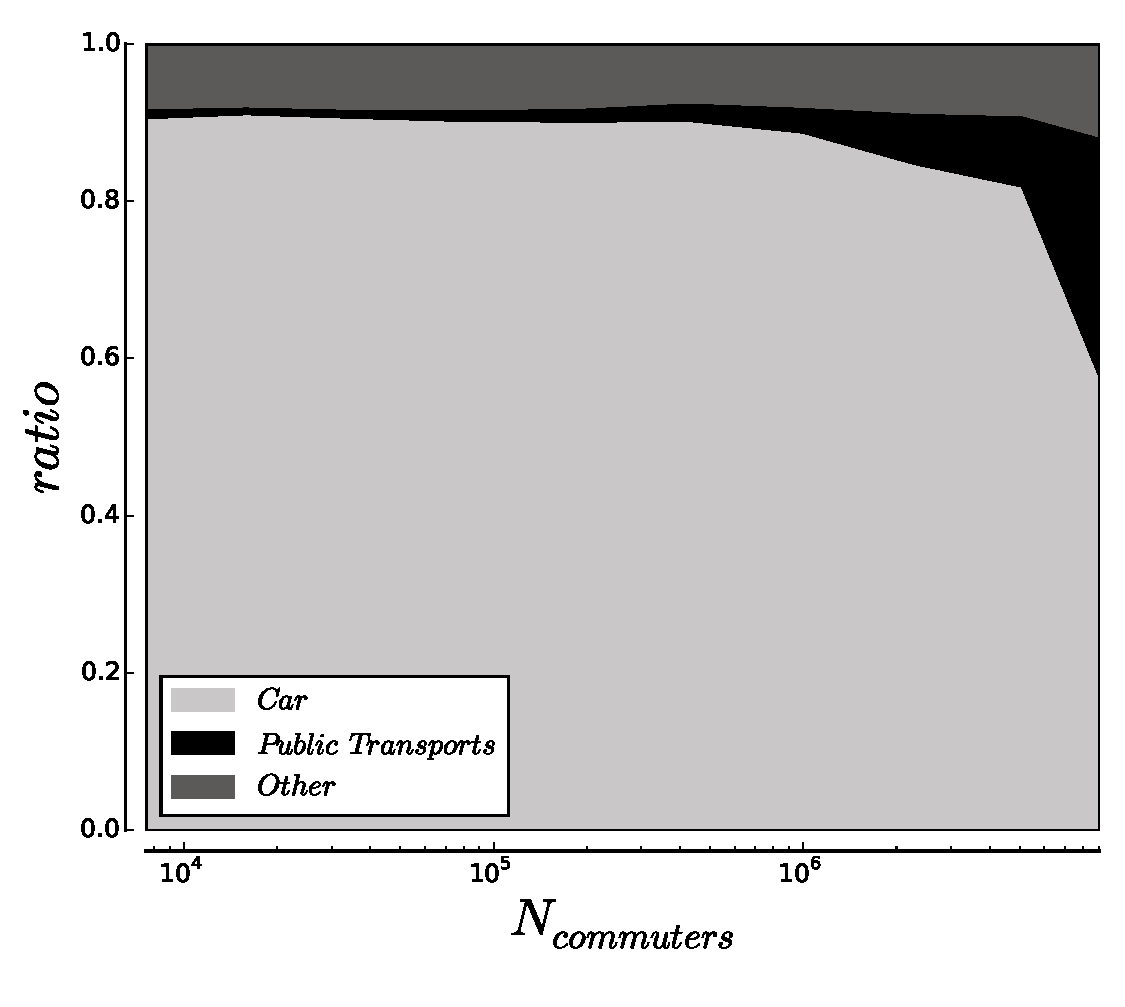
\includegraphics[width=0.8\textwidth]{gfx/chapter-monocentric/transportation_modes.pdf}
    \caption{{\bf Mode share in the US.} Importance of different transportation modes in US Metropolitan
    Statistical Areas, as a function of the number of commuters. Although the
proportion of individuals using public transportation or other modes (walking,
cycling, working at home) increases with population size, cars stay the dominant
mode of transportation everywhere. Data from the 2013 American Community
Survey.\label{fig:transportation_mode}}
\end{figure}


Another possible (but non-trivial) extension to the model is linked to the
second limitation stated above. Adding an income structure into the model (and
rules concerning the interaction of individuals) could allow us to explore the
spatial patterns of segregation, and see whether they can be understood from
basic economical choices alone~\cite{Gauvin:2013}. We considered this avenue
during this thesis, and realised there was very little of the empirical
knowledge on segregation could be used to test a model. This led us to working
on the material presented in Part~\ref{part:stratification} of this thesis.\\



\medskip

\section{Shadows in the empirical picture}
\label{sec:empirical}

\subsection{delineating and counting centers}
\label{sub:measuring_the_number_of_centers}

There is also some work left to be done on the empirical side. Although
non-parametric methods are an improvement over the previous parametric methods,
we are yet to understand what the meaning of the obtained centers is. 


In particular, a problem that remains with non-parametric methods is that, no
matter the distribution of employment, population, etc. into the areal units,
the method will output a number. For instance, let us consider the extreme case
of a city where employment is uniformly distributed in space, so that the
employment density is uniform. In this situation, the LouBar method would tell
us that the number of centers is equal to the number of areal units. Yet, can we
really talk about centers in this case? Most would (rightfully) object. But on
what ground?

The difficulty resides in that we do not know what we mean exactly when we talk
about centers: do they reflect an objective reality, or are they a mere artifact
of the way our brains process information? In the latter case, parametric
methods will do just fine. In the former case means we need to understand
what we talk about when we talk about centers. Ironically, more than $15$ years
after the publication of McDonald's seminal paper~\cite{McDonal:1987}, we are
still pondering over the same original question.\\


A further shortcoming of the most recent (distribution-based) methods is that
they do not consider the spatial arrangement of the areal units involved. This
can be problematic, especially when the method identifies as centers areal units
that are contiguous. 

We show an example of such situation on Fig.~\ref{fig:hotspots_boston}. We use
the LouBar method~\cite{Louail:2014} to extract the employment hotspots in the
Boston, MA MSA using data from the 2000 Census. As one can see, several of the
identified hotspots are contiguous. Should we still count them as separate
hotspots? Or should we consider that all contiguous hotspots are part of a
larger hotspots that encompasses them all? 

\begin{figure}[!h]
    \centering
    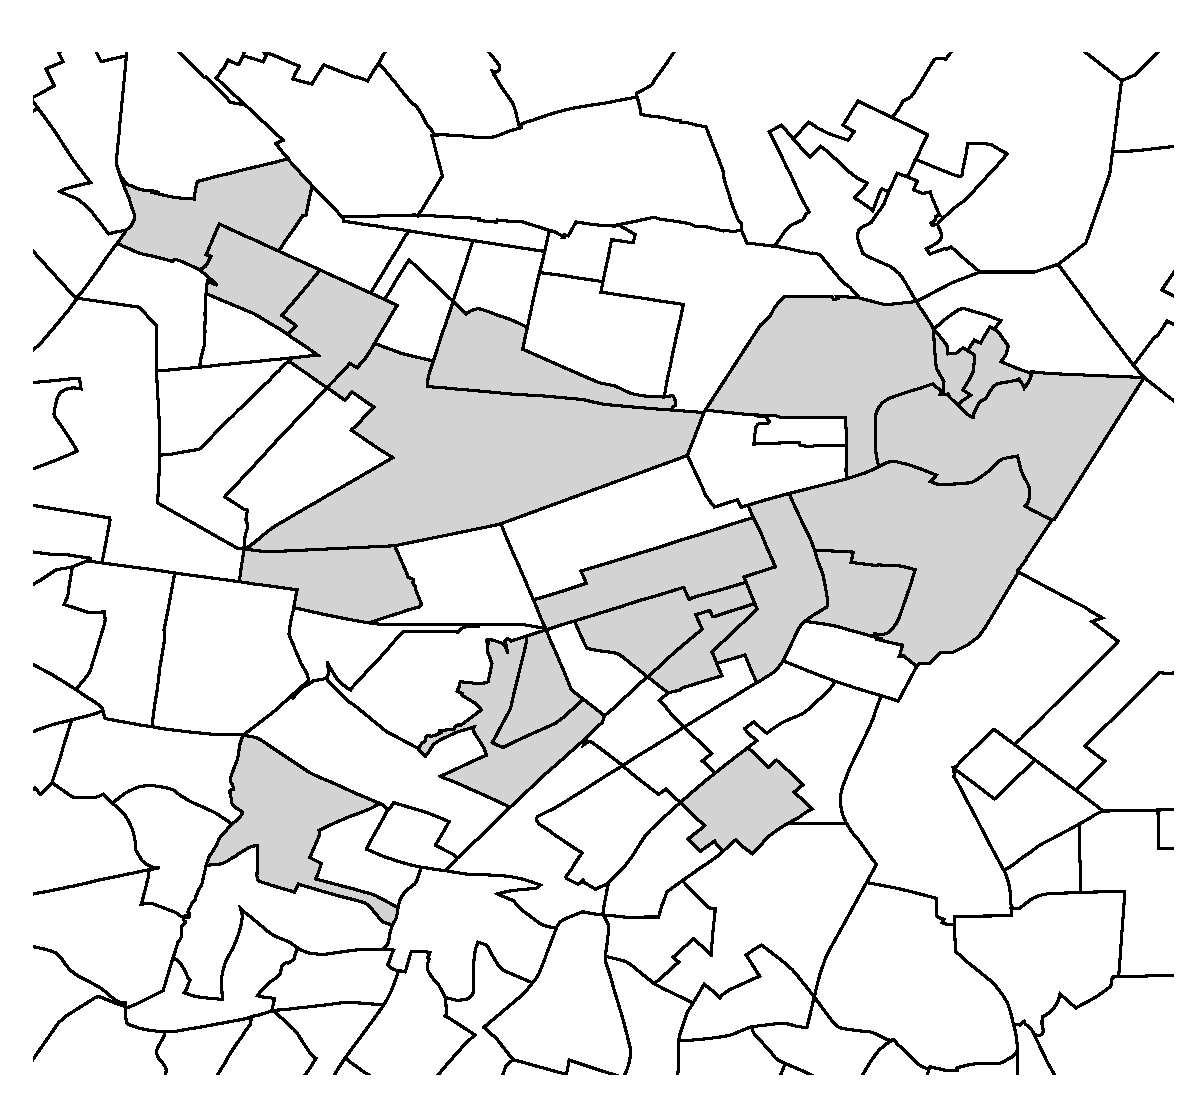
\includegraphics[width=0.75\textwidth]{gfx/chapter-monocentric/hotspots_boston.pdf}
    \caption{{\bf Subcenters and contiguity.} The census tracts of downtown Boston, MA in the US. In light grey,
    the census tracts that are identified as employment hotspots by the LouBar
method. Although the method designates all light grey tracts as different hotspots,
many of them are contiguous. We can wonder whether such contiguous
hotspots are, in fact, part of a larger hotspot that would include all of them.
This plot was generated using the 2000 Census tract-to-tract
commuting flows and the 2000 Census tracts geometry.\label{fig:hotspots_boston}}
\end{figure}


The results of the methods provided in the introduction should not be thrown
away altogether, though. The number of centers they provide probably does not
reflect the `real' number of centers (if there is such a thing) in a particular
city. But, assuming that different cities exhibit similar structures, they
should still provide values that are coherent across different urban areas, and
are thus useful for \emph{comparison} purposes.\\


\subsection{Beyond polycentricity?}
\label{sec:beyond_polycentricity}


\subsubsection{The dispersed city}
\label{sub:the_dispersed_city}

As we saw in Chapter~\ref{chap:monocentric_introduction}, the concept of the
monocentric city got replaced with the more elaborate polycentric hypothesis. It
is, however, not the end of the story. Gordon and Richardson, in a
provocative article~\cite{Gordon:1996}, argue that cities are dispersed more
than they are polycentric. Indeed, studying the employment density in Los Angeles,
they found that the centers they defined based on density only contained $17\%$
of the total employment. Hardly a polycentric situation!  Of course, we can
wonder whether Gordon and Richardson's results are an artefact of the choice of
their case study --Los Angeles, famous for its sprawl-- or the particular method
they used to compute the number of centers. We thus plot on
Fig.~\ref{fig:concentration_loubar} the ratio of the total number of individuals
that is contained in the centers defined by the LouBar method. The results are
striking: only a few, small metropolitan area reach the mark where $50\%$ of
individuals (employees or residents belong) to a designed center. Worse, cities
seem to be on average more dispersed as they are bigger.\\

\begin{figure}
    \centering
    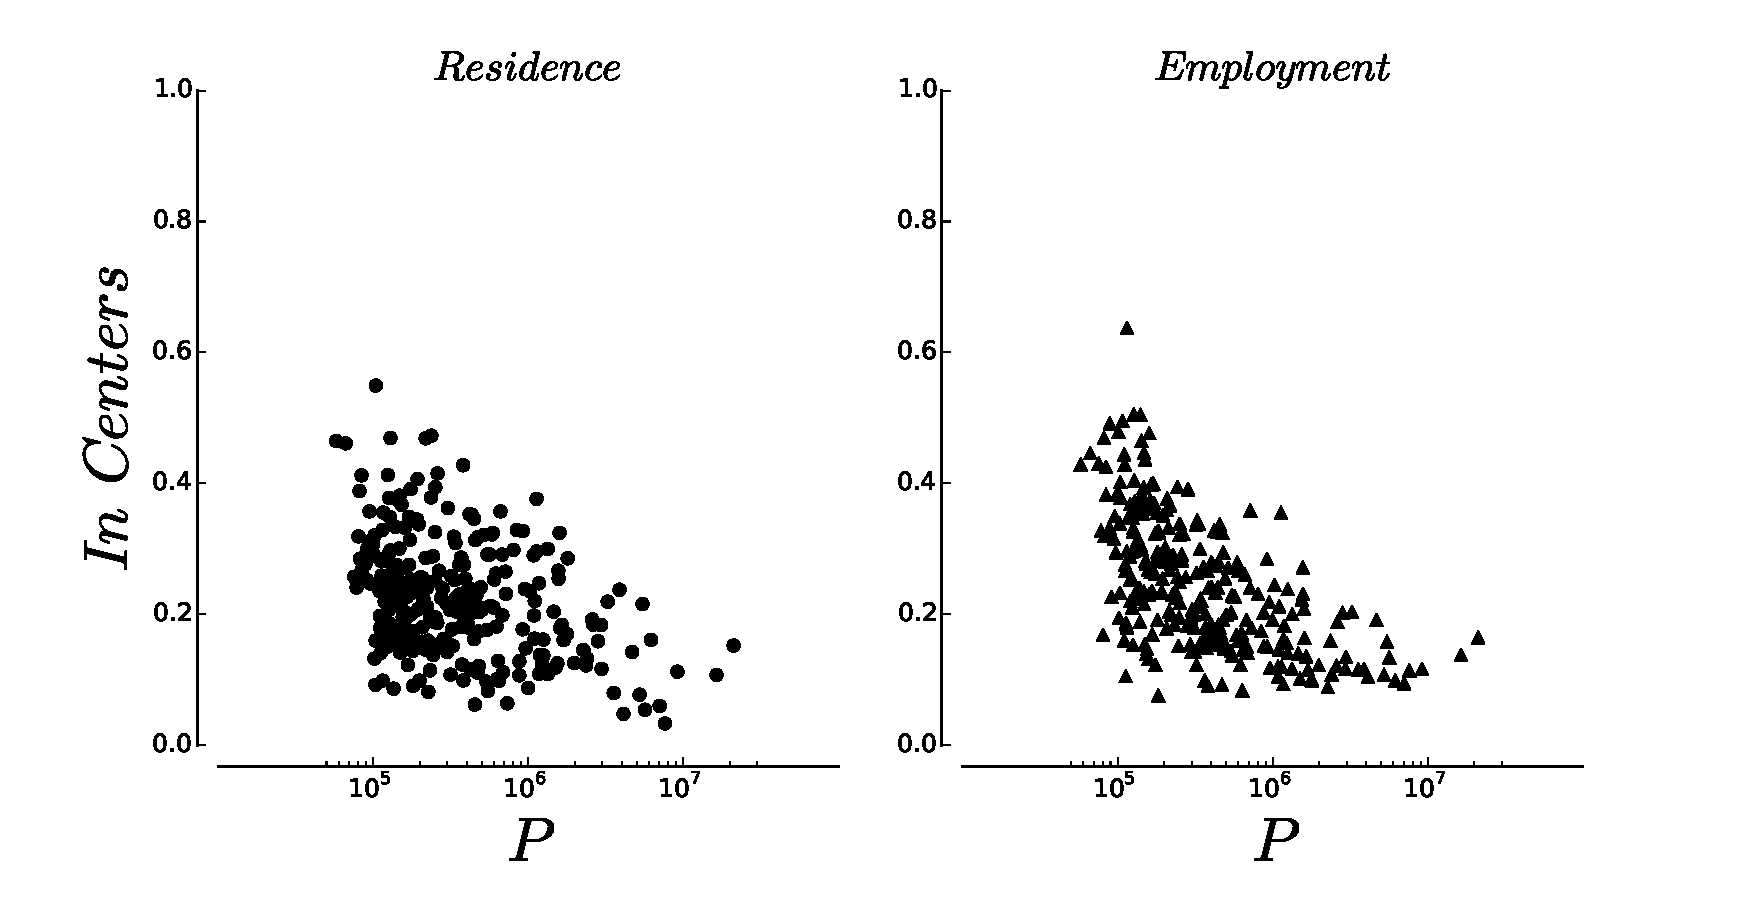
\includegraphics[width=1\textwidth]{gfx/chapter-monocentric/concentration_loubar.pdf}
    \caption{{\bf Concentration in subcenters.} (Left) Ratio of the total
    residential population in US MSAs that lives in the centers identified by the LouBar
method. (Right) Ratio of the total number of employees in US MSAs that works in the centers
identified by the LouBar method. Overall, cities are very dispersed, with only a
few cities having more than $50\%$ of their workforce or residential population
living in centers, confirming the results of Gordon and
Richardson~\cite{Gordon:1996}. Data were obtained for the 2000 US Census, the
figure was prepared using Python.\label{fig:concentation_loubar}}
\end{figure}

The lesson that should be learned from the article by Gordon and Richardson is
that the notion of polycentricity is \emph{also an hypothesis} on the spatial
structure of densities. While it is arguably more involved than the monocentric
hypothesis, it does indeed implicitly impose some structure onto the data. The
process itself of counting centers implies that these centers exist, that there
is an element of reality attached to what we call centers. A quick look on the
3D plot shown on Fig.~\ref{density_3d} should convince the reader that the world
is not as simple as the way we picture it. For intance, while employment
densities indeed exhibit strong peaks that are easily distinguishible (although
that is arguable for Houston), the same cannot be said for population densities.
The point, I argue, is not that the monocentric or the polycentric model are
wrong altogether. The problem lies in the lack of appropriate tools to describe
a density spatial profile, in the fact that there is no `one size fits all'
method of analysis. Indeed, the exploratory tools presented above, try to fit a
certain model of the city to the actual data, be it monocentric or
polycentric.

\subsubsection{Quantifying Urban form}
\label{sub:urban_form}

This problem is in fact very general, and pertains to the field of spatial
analysis (including spatial statistics). Finding centers indeed amounts to
finding the proper way to describe a density profile at a meso-scale level and
to devising proper methods to detect the salient feature of this spatial
pattern. The collection of tools and methods to describe the structure
of density patterns in cities consitutes the sub-field of urban
form~\cite{Tsai:2005,Schwarz:2010,LeNechet:2015} and reaches far beyond the
determination of subcenters.

We have focused in this part on the \emph{morphological} aspect of urban form,
as most of the preceding studies. We ackowledge however the existence of a
\emph{functional} aspect (see~\cite{Berroir:2008}), which takes the attraction
range of employment subcenters into account, in addition to the raw number of
employees. Mixing employment densities and the property of the flows to the
center may indeed lead to a better understanding of what a center really is.

Despite important progress, the tools provided by spatial analysis do not yet
provide a satisfactory picture. However, such tools would also help to describe
the spatial patterns of segregation that we study in
Part~\ref{part:stratification} of this manuscript.

\section{Summary}
\label{sec:summary}

In this part, we have presented an historical overview of the monocentric
hypothesis for the structure of cities, and how the view has progressively
shifted towards the picture of a more distributed, polycentric organisation.
Starting with indirect evidence for a polycentric picture, several methods were
then naturally proposed to directly measure the number of centers, from the
first parametric methods to the more recent non-parametric methods. Observing
evidence for an increased polycentricity with population size, we then wondered
what were the possible explanations for this phenomenon. We proposed an
out-of-equilibrium model of city growth that predicts the necessary emergence of
secondary centers as populations grows, and a sublinear increase of the number
of subcenters with population---both verified on empirical data, across
different countries, for several city definitions.

In the next part, we will continue our journey with another, seemingly unrelated
topic: scaling relationships. We will start with an historical perspective on
scaling, showing that scaling relationships did in fact precede Quantitative
Geography, and we will provide a non-exhaustive review of the empirical results.
We will then be ready to show how, using the model exposed in this chapter, we
can understand the scaling relationships related to mobility in cities. We will
then conclude on a reflection of what scaling relationships can and do tell us
about cities, and highlight their shortcomings.
